\documentclass[aspectratio=169,xcolor={rgb}]{beamer}

\usepackage[T1]{fontenc}
\usepackage{lmodern}
\usepackage{microtype}
\usepackage{graphicx}
\usepackage{booktabs}

% The theme lives in the Quarto extension folder. Point LaTeX there for the
% .sty files and the logos: _extensions/nmbu/ in the template repo,
% _extensions/edsandorf/nmbu/ after `quarto add` or `init-beamer`.
\makeatletter
\def\input@path{{_extensions/nmbu/}{_extensions/edsandorf/nmbu/}}
\makeatother
\graphicspath{{_extensions/nmbu/}{_extensions/edsandorf/nmbu/}}

\usetheme{nmbu}

% References
\usepackage[backend = biber, citestyle = authoryear-comp]{biblatex}
\addbibresource{references.bib}

% Title information
\title{This is my presentation}
\subtitle{With a subtitle}

\author{John Lennon \inst{1} \and Paul McCartney \inst{1} \and George Harrison \inst{1} \and Ringo Starr \inst{2} \and Another Author \and Yet another author}
\institute{\inst{1} First institute \and \inst{2} Second institute}

\date{2026-11-27}

% LOGOS ----
% This is a comma separated list of logos to include at the bottom of the slide.
\newcommand*{\logos} {
    gfx/logo-nmbu,
    gfx/logo-aacsb-accredited
}

% BEGIN PRESENTATION -----
% The slides match NMBU-example-quarto.qmd one to one, so the two decks can be
% compared page by page. The plots come from figs/make-figures.R.
\begin{document}

\begin{frame}
  \titlepage
\end{frame}

\begin{frame}{Outline}
  \tableofcontents
\end{frame}

\section{Introduction}

\begin{frame}{Informative titles state the point of the slide}
  \begin{itemize}
    \item Minimal text on the slide
    \item The interpretation goes in the speaker notes
  \end{itemize}
  \note{Speaker notes are hidden in the PDF by default. Show them with
  \texttt{\textbackslash setbeameroption\{show notes on second screen=right\}}.}
\end{frame}

\begin{frame}{Math examples and a really really really long headline that hopefully will break across}
  \begin{equation}
    \hat{H}\Psi = E\Psi
  \end{equation}
  \begin{equation}
    \varepsilon \otimes \Omega
  \end{equation}
\end{frame}

\section{Methods}

\begin{frame}{Outline}
  \tableofcontents[currentsection]
\end{frame}

\begin{frame}{The MNL model}
  \begin{equation*}
    \Pr(i_{nit} \mid \beta) = \frac{\exp(\beta X_{nit})}{\sum_{j=1}^{J}\exp(\beta X_{njt})}
  \end{equation*}
  where
  \begin{itemize}
    \item $\beta$ is a vector of parameters to be estimated
    \item $X_{nit}$ are the levels of the attributes
  \end{itemize}
\end{frame}

\begin{frame}{Another frame with some equations}
  \begin{equation*}
    \begin{split}
      \int_2^4\frac{1}{x^2}dx &= \int_2^4 x^{-2}dx\\
      &= \left[\frac{1}{-2+1}x^{-2 + 1}\right]_2^4\\
      &= \left[-\frac{1}{x}\right]_2^4\\
      &= -\tfrac{1}{4} - \left(-\tfrac{1}{2}\right)\\
      &= -\tfrac{1}{4} + \tfrac{1}{2}\\
      &= \tfrac{1}{4}
    \end{split}
  \end{equation*}
\end{frame}

\begin{frame}{Blocks}
  \begin{block}{Standard block}
    This is a standard block.
  \end{block}

  \begin{exampleblock}{Example block}
    This is an example block.
  \end{exampleblock}

  \begin{alertblock}{Alert block}
    This is an alert block.
  \end{alertblock}
\end{frame}

\section{Graphics}

% The example images below ship with the mwe package in TeX Live/MiKTeX.
\begin{frame}{A full-slide graphic}
  \fullslidegraphic{example-image-16x9}
\end{frame}

\begin{frame}{A full-slide graphic still fits when the frame title is long enough to break across two lines}
  \fullslidegraphic{example-image-golden}
\end{frame}

\begin{frame}[plain]{A plain frame has no footline, so the graphic can use that space too}
  \fullslidegraphic{example-image-golden}
\end{frame}

\begin{frame}{Two graphics side by side at full height}
  \setfullslideheight
  {\centering
    \includegraphics[height=\fullslideheight]{example-image-golden-upright}\hspace{1em}%
    \includegraphics[height=\fullslideheight]{example-image-a}\par}
\end{frame}

\begin{frame}{A row of photos with different aspect ratios}
  \begin{columns}[T]
    \begin{column}{0.32\textwidth}
      \coverimage{\linewidth}{3.4cm}{example-image-16x9}
    \end{column}
    \begin{column}{0.32\textwidth}
      \coverimage{\linewidth}{3.4cm}{example-image-golden-upright}
    \end{column}
    \begin{column}{0.32\textwidth}
      \coverimage{\linewidth}{3.4cm}{example-image-1x1}
    \end{column}
  \end{columns}
\end{frame}

\section{Results from R}

\begin{frame}[fragile]{Code shown on a slide}
\begin{verbatim}
model <- lm(dist ~ speed, data = cars)
coef(model)
\end{verbatim}
\begin{verbatim}
(Intercept)       speed
 -17.579095    3.932409
\end{verbatim}
\end{frame}

\begin{frame}{Regression output as a table}
  \centering
  \begin{tabular}{lrrrr}
    \toprule
                & Estimate & Std. Error & t value & Pr(>|t|) \\
    \midrule
    (Intercept) & -17.579  & 6.758      & -2.601  & 0.012    \\
    speed       & 3.932    & 0.416      & 9.464   & 0.000    \\
    \bottomrule
  \end{tabular}
\end{frame}

\begin{frame}{Stopping distance rises with speed}
  \centering
  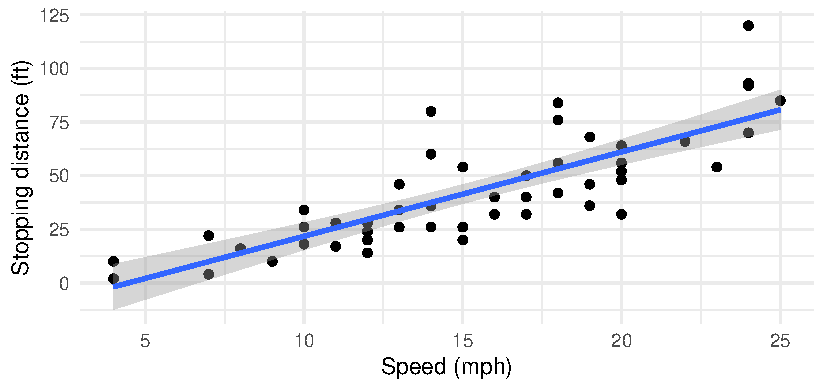
\includegraphics{figs/stopping-distance}
\end{frame}

\begin{frame}{A plot next to text}
  \begin{columns}
    \begin{column}{0.55\textwidth}
      \centering
      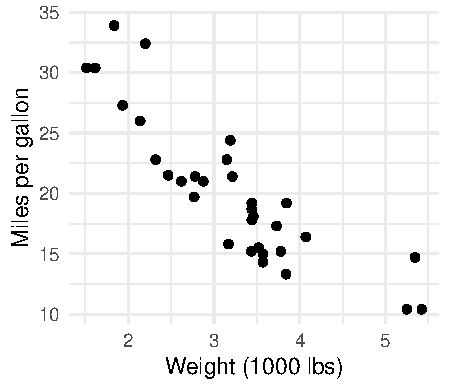
\includegraphics{figs/mpg-weight}
    \end{column}
    \begin{column}{0.45\textwidth}
      \begin{itemize}
        \item Heavier cars drive fewer miles per gallon
      \end{itemize}
    \end{column}
  \end{columns}
\end{frame}

\begin{frame}{Text with references}
  Some random text with references in the footnote \footfullcite{sandorf_exploring_2025} or in
  parentheses \parencite{sandorf_ponderous_2022}.
\end{frame}

\begin{frame}[allowframebreaks]{References}
  \printbibliography
\end{frame}

\end{document}
